% vim: set tw=0:
\documentclass{beamer}
\usepackage{graphicx}
\usepackage{hyperref}
\hypersetup{pdfborder={0 0 0 0}}

% Reasonable themes:
% Antibes Bergen Berkeley Berlin Frankfurt Goettingen Ilmenau Luebeck Malmoe
% Montpellier PaloAlto Rochester Singapore Szeged Warsaw bars boxes
% compatibility default lined plain shadow sidebar split tree
% And these ones include the author's name on every slide:
% Berkeley

% Declare themes.
\mode<presentation>
\usetheme{UWHEP}

% Personal macros.
\newcommand{\email}[1]{{\texttt #1}}
\newcommand{\newframe}[1]{\section{#1}
    \frametitle{\sc{#1}}}
\newcommand{\subframe}[1]{\subsection{#1}
    \frametitle{\sc{#1}}}
\newcommand{\supers}[1]{\ensuremath{^\textrm{#1}}}
\newcommand{\subs}[1]{\ensuremath{_\textrm{#1}}}
\newcommand{\ca}{\ensuremath{\sim}}
\renewcommand{\email}[1]{\href{mailto:#1}{\nolinkurl{#1}}}

% Author information.
\title{T2 Status}
\author[Maier, Mohapatra]{
    Will Maier \and Ajit Mohapatra\\
    {\tt wcmaier@hep.wisc.edu}\\
    {\tt ajit@hep.wisc.edu}}
\institute[Wisconsin]{University of Wisconsin - High Energy Physics}
\date{2009.12.08}
\logo{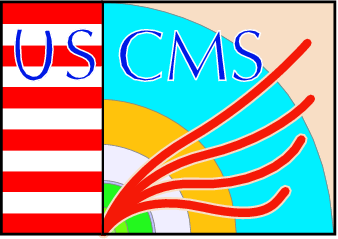
\includegraphics[height=0.6cm]{../../../Graphics/USCMS_logo.png}\hspace{.1cm}
\includegraphics[height=0.75cm]{../../../Graphics/UW_logo.png}}

\begin{document}

\begin{frame}
    \titlepage
\end{frame}

%\section{Overview}
%\begin{frame}
%    \tableofcontents
%\end{frame}

\section{Facilities}
\subsection{Software and Storage}
\begin{frame}
\frametitle{}

\begin{itemize}
	\item Order for perfSONAR machines finally went through and they're now shipping
	\item Trying to order PNFS server replacement; stuck in purchasing\ldots{}
	\item Moving nested directories in PNFS caused {\tt OSM not found} errors
	\begin{itemize}
		\item User tried to rearrange after CRAB dumped files in an unexpected location
		\item No alternative but to delete the broken files?
	\end{itemize}
	\item Cleaned up replicas with bad statuses in dCache; \ca{}10k files, several TB of disk
	\item Wrote a GIP plugin to report dCache storage
	\item Implemented {\tt dcache\_df} based on info service's XML
	\begin{itemize}
		\item \url{http://code.hep.wisc.edu/dcache-tools}
	\end{itemize}
\end{itemize}
\end{frame}

\subsection{Production and Monitoring}
\begin{frame}
\frametitle{}
\begin{itemize}
	\item JobRobot: OK
	\item SAM: OK
	\item RSV: OK
	\item PhEDEx:
	\begin{itemize}
		\item 3\_2\_9 is stable
		\item {\tt BlockDownloadVerify} still has the dataset consistency check bug
		\begin{itemize}
			\item Loops indefinitely while making the check; Tony will fix it soon
		\end{itemize}
		\item More T2/T3 links commissioned via LoadTest
		\item Usual MC subscriptions for local users
	\end{itemize}
	\item MC Production:
	\begin{itemize}
		\item Summer09 production continues for 7TeV and 10TeV
		\item We have hit the 1B mark for FullSim events, still some more left to do
		\item We produced \ca{}50M high priority 900 GeV and 2360 GeV samples with the latest detector conditions and beamspot values
		\item Heavy Ion requests are now integrated to the official MC production
	\end{itemize}

\end{itemize}
\end{frame}

\end{document}
